\documentclass{hw}

\usepackage{minted}

\begin{document}
\makeheader{1}

\begin{enumerate}
\item Dr. Martin has emailed you the data set, hmwk1.txt, which gives the time evolution of a certain
quantity of interest to him. Using R, plot the original data. In addition, using R’s ma() function, plot a
smoothed version of the data. What attribute of the original data is hidden by referring only to the
smoothed data?
\begin{quote}
\inputminted{r}{num_one.R}
The output of the above code is\\
\begin{minipage}{0.5\textwidth}
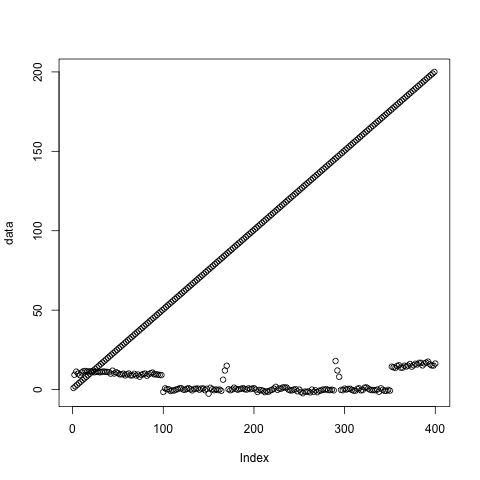
\includegraphics[scale=0.4]{01data_plot}
\end{minipage}
\begin{minipage}{0.5\textwidth}
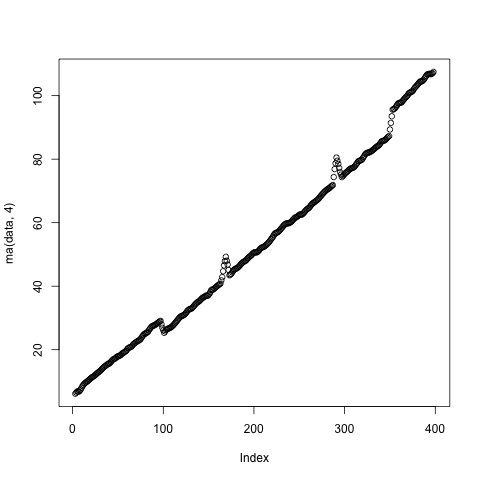
\includegraphics[scale=0.4]{01data_smoothed}
\end{minipage}
When the data is smoothed, the outlying points are lost.
\end{quote}

\newpage
\item Dr. Martin has emailed to you the data set, co2.txt. The data represents 16 years of collecting
monthly $CO_{2}$ data on the island of Hawaii, with the first year of $CO_{2}$ starting in January of
1958. a) Using R, plot the data. b) Using R’s stl() command, plot the 1. trend, 2. seasonal, and 3.
irregular components of the data.
\begin{quote}
\inputminted{r}{num_two.R}
\begin{minipage}{0.5\textwidth}
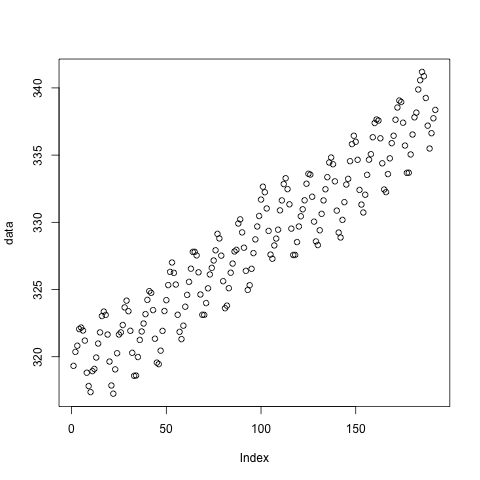
\includegraphics[scale=0.4]{02data_plot}
\end{minipage}
\begin{minipage}{0.5\textwidth}
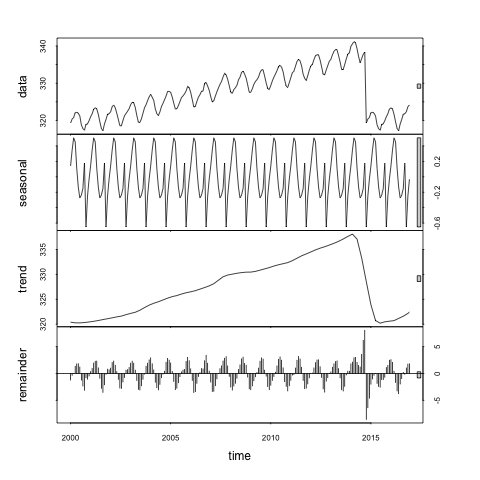
\includegraphics[scale=0.4]{02seasonal}
\end{minipage}
\end{quote}

\newpage
\item 
\end{enumerate}
\end{document}
